
\chapter{Haskell-Python}
\label{chap:hs}

% TODO !!! Give credit to the developers !!!

Haskell-Python\cite{haskellpython}
is an interpreter for a language similar to Core, we call it Core' here.
This interpreter is the base for our JIT compiler. In this section we descripe a 
syntax and an informal semantics for Core', as well as a description of the 
interpreter.


\section{Syntax}
\label{sec:syntax}

Although Core' does not have a syntax, we define one here, as we use it later 
to show how Core is translated to Core'.

In the following grammar, the '[' and ']' symbols are used to mean that
anything between can be repeated, 0 or more times. We use '[' and '$]^+$' to 
mean that the pattern can be repeated 1 or more times. Non-terminals are 
written with italic font throughout the paper.
See figure \ref{gr:coresyn} for the full syntax.

\begin{figure}[H]
\centering

\begin{grammar}
<Constructor> ::= const( <Symbol>, [ <Value> ] )

<Function> ::= func( <Name>, [ <Rule> ]$^+$ )

<Rule> ::= rule( [ <Value> ]$^+$ = <Exp> )

<Exp> ::= exp( <Value> )
     \alt exp( <Prim-Function> )
     \alt exp( <Function> )
     \alt exp( <Application> )

<Application> ::= app( <Exp>, [ <Value> ] )

<Literal> ::= str( <String> )
	 \alt num( <Number> )
	 \alt char( <Character> )

<Value> ::= <Literal>
       \alt <Constructor>
       \alt <Variable>

<Variable> ::= var( <Name> )

<Symbol> ::= An identifier that can be matched against.

<String> ::= A list of characters

<Number> ::= A number

<Character> ::= A character

<Prim-Function> ::= A function that is implemented at the machine level.

\end{grammar}

\caption{Core' syntax}
\label{gr:coresyn}

\end{figure}

\section{Informal semantics}

The Launchbury semantics is an operational semantics for 
lazy evaluation, which the Core' interpreter follows rather closely. 
This section will be a brief introduction to the semantics of the interpreter.
For a introduction to 
the Launchbury semantics, see \cite{launchbury1993natural}. 

A Core' program is evaluated by reducing the main application to WHNF 
(Weak Head Normal Form). A construct is in WHNF if it can't be
reduced any further.

\subsection{Value}
A Value can be a Literal, Constructor, or a Variable. All values are in WHNF.
% What about the implementation of low-level types ???

\subsection{Constructor}
A Constructor is just a Value, containing other Values.

\subsection{Function}
A Function is a named collection of Rules. It must contain at least one Rule.

\subsection{Rule}
A Rule is a list of Values, followed by an Expression. Note that the only Variables
that are in scope in the Expression, are those defined in the list of Values within 
the Rule.

\subsection{Expression}
An Expression can be a Value, a Primitive-Function, a Function, or an Application.
An Expression is in WHNF if it does not contain any unevaluated Applications.

\subsection{Application}
An Application represents the evaluation of a function with variables applied to it.
An Application is not in WHNF.

When the Application is evaluated, the arguments are matched against the list of 
Values contained in the list of Rules. 
When the arguments match a Rule, the Expression contained in this rule is evaluated. 
The Variables in the expression are replaced by the values that matched the same-name
Variables in the Value list. Then the Expression is evaluated, returning a new Value.

\subsection{Literal}
A Literal is a Value such as an integer, a string or a character.





\section{Evaluation}

The evaluation of a Core' Application is performed on a stack called the
todo-stack. All the objects handled by the interpreter has a function called
step. This function takes the todo-stack as an argument, and performs an
interpretation step, with the goal of moving the object towards a state
closer to evaluated. The step-function returns a new Value object and a
stack object. The todo-stack can grow or shrink, depending on the state of
the object "stepping".

The todo-stack consists of two types of objects, the UpdateStackElement,
and the CopyStackElement. 

The CopyStackElement is created by an Applications eval\_after function. The
eval\_after function is called when an Application is attempted applied, but
the arguments need to be evaluated first. Alternatively, the eval\_after
function is called when an Application is evaluated and returns a new
Application (A higher-order function). 

The step function of the CopyStackElement takes a argument called value,
and returns a new Application with one of the Applications arguments
replaced by the value-argument. Or the Applications Function is replaced
by the value-argument.

The UpdateStackElement contains a Thunk (an unevaluated Application). The
The step function of the UpdateStackElement returns the Application contained
in the Thunk, and the next part of the stack (the stack is implemented as a
linked list).

\begin{comment}

\section{Evaluation}

A Core' program is executed by reducing a main Application to WHNF.

%\subsection{The evaluation stack}

When an Application is evaluated; two things can happen. If it does not contain
other unevaluated Applications it can be evaluated directly. However, if it does
contain unevaluated Applications, it is added to the evaluation stack, and its 
arguments are added on top of it, with any Applications turned into a Thunk 
(a suspended evaluation). Evaluation proceeds from the top of the stack.
untill its unevaluated parts have become evaluated (reduced to WHNF), and the
Application itself is ready to be evaluated.
See figure \ref{fig:sketch} for a concept sketch.

%it's unevaluated parts is pushed onto an 
%evaluation stack. The stack can contain two kinds of elements, a CopyStackElement,
%and a UpdateStackElement. Evaluation is always continued from the head of the stack.

% An UpdateStackElement contains a Thunk. ?

% A CopyStackElement contains an Application. ?

%\subsection{Thunk}

%A Thunk is a suspended evaluation, in effect, an unevaluated function application.

\end{comment}

\section{Example Core' program}

Fibonacci:

\begin{lstlisting}
func( "fib", [
	rule( lit(0) = num(1) )
	rule( lit(1) = num(1) )
	rule( var(x) = 
		app( +, [
				app( fib, [ app( -, [var(x), num(1)] ) ] ), 
				app( fib, [ app( -. [var(x), num(2)] ) ] )
			])
		)
	])
\end{lstlisting}

Note that "+" and "-" refers to the primitive implementations of addition 
and subtraction respectively.


\begin{comment}

\section{Implementation}

The description of Haskell-Python can be 
logically divided into two parts; "the way programs are 
represented", and "the way programs are evaluated".

\subsection{Program representation}

Programs are represented by a set of Classes; Value, Constructor, Function, Rule, 
PrimFunction, Var, Application (Additional classes are created for Constructor
and Application for various number of arguments through the classes ConstructorN 
and ApplicationN). The syntax defined in \ref{sec:syntax} corresponds very much
to the organization of classes in the interpreter. 

A Value is a base class for objects in WHNF. A Constructor inherits from Value.
The Function and PrimFunction also inherits from Value (indirectly 
via inheritance of AbstractFunction). Functions are Values because they can't 
be reduced any further (they are already in WHNF).

% Can a constructor contain all HaskellObjects ??? Why ?
The Constructor classes can contain Values as their arguments, however, since
a Constructor is itself a Value, it can not have unevaluated applications as
arguments. The Constructor is characterized by a Symbol. A Symbol is simply
a name that can be matched by identity.

The PrimFunction class represents a function that is not implemented in 
Haskell, but is implemented at the machine level.

The Function class represents a user-defined function.

A Var is substituted with a NumberedVar when a Rule is created. This simply
means that the new NumberedVar is only in scope within the Rule.

\subsection{Program evaluation}

A Substitution is the body of a Function with numbered variables 
(NumberedVar) substituted by values.

The evaluation of a program is done by a function, main\_loop. The function
takes a variable 'expr' as argument, and reduces it to WHNF. The reduction is done
by continously pushing/popping from the evaluation stack. 

The evaluation stack is represented by a base class, StackElement. Two other
classes inherits from this class, UpdateStackElement and CopyStackElement. Note that
the stack is implemented by a linked list (each StackElement points to the next).

% TODO ! Describe how recursion works in this same way.
\begin{sidewaysfigure}
\begin{figure}[H]
\centering
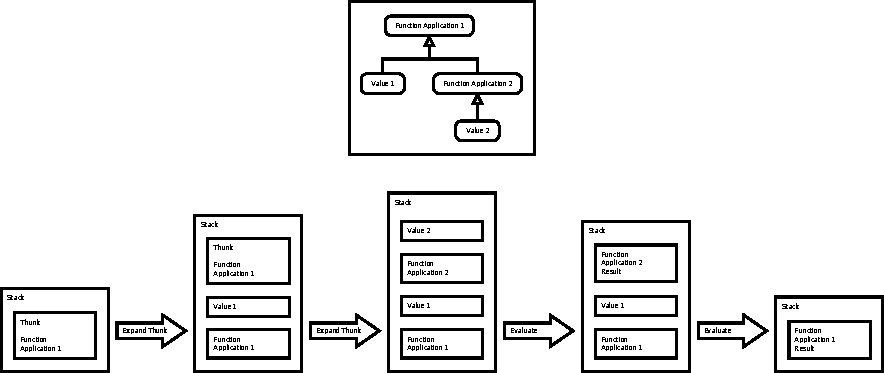
\includegraphics[width=\textheight]{../diags/eval-stack.pdf}

\caption{Overly simplified concept sketch of the evaluation stack; 
when the first Application is to be evaluated, it is discovered that it
contains unevaluated expressions. The Application is turned into a Thunk.
The Thunk is then popped from the stack, and the Application is added to
the stack, the Application arguments are popped on the stack with any 
Applications turned into thunks. The top of the stack is again a Thunk.
The same routine is performed on the new Thunk, until the expression top
Application can be reduced to a Value. After this, the initial Application
can also be reduced to a Value.
}
\label{fig:sketch}

\end{figure}
\end{sidewaysfigure}

\end{comment}

\section{Extensions}

This project involved extending Haskell-Python to a full Haskell interpreter 
through the use of GHC.

\subsection{GHC usage}

% TODO

By using GHC to compile the Haskell programs and dump its intermediate
format to a file, we can effectively turn Haskell-Python into a full
Haskell compiler. However, the format dumped by GHC is External-Core.

We turn External-Core into JSCore with a Haskell program called "core2js".
JSCore is a JSON compliant representation of external-core. This means that
we can parse JSON and get a representation we can easily traverse when building
the AST (Abstract Syntax Tree) for the Core' interpreter.

\subsection{Module system}

% TODO
A module system was implemented for the interpreter. A module object contains
a dictionary for variables, type-constructors and data-constructors. The 
"library" contains a dictionary of modules. This structure corresponds to the
module hierarchy used by GHC.

\subsection{Parser}

% TODO

The parser is implemented using some of the PyPy parsing tools. A simple 
JSON grammar is described in EBNF form in a Python string. This string
is then parsed by the PyPy tool and a parser is created. By using this JSON
parser and traversing the resulting datastructure, we build the AST for the 
interpreter. See section \ref{chap:rewrite} for a detailed description of 
the parser and the Core to Core' mapping.

\subsection{Primitives}

% TODO
The Primitive values extend the Value class. Primitive functions handle
these values.
See section \ref{chap:prims} for a more in-depth discussion of the
library and primitives.

